\chapter{Background}
\label{ch:background}
% This chapter will present the necessary background information for this thesis. First, we define some basic terminology that will be used throughout this thesis. Next, ...
In this chapter we will explain the background information needed to understand the thesis. We start by looking at different sources that show which programming language is popular. Then we will look at the a source for programming languages that have the same functionality. After that we will look at a system that could be used for measuring the energy consumption. Finally we will delve into the different statistical tests used. 

\section{Programming languages}
When looking into what the most used/popular programming languages are we find different results. Here are four different sources with their own opinion of what the most used/popular programming languages are.\\

Git-hub is a version control system where multiple programmers collaborate in a project. They looked at the amount of pull requests made for that language \cite{zap:2019}. The thought was that the language that programmers work a lot with on git is the most popular, but this is based on only the public repositories. In the first quarter of 2019 the top ten according to this method is JavaScript, Python, Java, Go, C++, Ruby, PHP, TypeScript, C\# and C. \\

Indeed is a job search site. They looked at the percentage of jobs with a programming language in their name in the tech software category \cite{ray:2018}. Thus the more job offering for a programming language the more popular that programming language is. The problem with this method is that job offerings do not show how many people work with a programming language, but only which programming language has a shortage in programmers. Based on data from September 2018 the top ten according to this method is Java, JavaScript, HTML, Python, C\#, C++, XML, Ruby, PHP and Perl.\\

TIOBE is a software quality company. They looked at the amount of hits they got when searching "[Language] programming" on a lot of different search engines \cite{tio:2019}. There are rules which a search engine needs to comply with for it to be used in the calculations and they also look a what type of hits they find to determine whether or not to use it in the calculations. The pitfall of this method is the favouritism for complex languages. When a language is more difficult to understand, more page of tutorials are needed and more questions about this language will be asked. As of April 2019 the top 10 according to this method is Java, C, C++, Python, Visual Basic .NET, C\#, JavaScript, SQL, PHP and Assembly language.\\

PYPL index stands for the PopularitY Programming Language index. They look at how many times a language tutorial is searched \cite{car:2019}. This method also has favouritism for complex languages, where programmers need to use the tutorials a lot because of the difficulty. Based on data form April 2019 the top ten according to this method is Python, Java, JavaScript, C\#, PHP, C/C++, R, Objective-C, Swift and Matlab.\\

\section{The computer language benchmark game}
The computer language benchmark game, also called the famous programming language shootout, compares different programs and languages based on their run time, memory usage, zipped program size and CPU usage \cite{gouy:2019}. The project features ten different problems with a variety of programs from different languages. Everyone can submit a program if it holds to the two requirements: follow the same algorithm and result in the correct output. This is important because we want to compare the way of writing a program and the difference in programming language, but not the difference in algorithm used. For every program featured, the correct output and required steps to compile the program are listed.\\

In the previous chapter we found that the energy consumption of a program is the sum of the CPU, memory and disk energy consumption \cite{acar2016impact}. To get a good view on what influences the energy consumption, our problems need to be diverse when it comes to these three categories. The problems that we looked into are called Binarytrees, Fannkuchredux, Fasta, Mandelbrot, Nbody, Revcomp and Spectralnorm. For the Binarytrees problem a lot of trees are allocated and deallocated in memory and thus this is a memory intensive task. The fannkuchredux problem does a lot of calculations on all permutations and is thus CPU intensive. The Fasta problem creates and saves a large DNA sequence and is memory intensive. For the Mandelbrot problem a large bitmap is saved and thus is it memory intensive. The Nbody problem models the orbit of Jovian planets and is CPU intensive. The Revcomp problem reads a DNA sequences line by line, transforms them and writes the result to output. Therefor the Revcomp problem is disk intensive. For the Spectralnorm problem a lot of calculations are done on a large matrix and is thus CPU intensive. A more extensive explanation of the problems can be found on the computer language benchmark game website \cite{gouy:2019}. An overview of category and problem is shown in table \ref{tab:problems}.

\begin{table}[h]
\centering
\begin{tabular}{|l|l|}
\hline
\textbf{Category} & \textbf{Problems}                           \\ \hline
CPU      & Fannkuchredux, Nbody, Spectralnorm \\ \hline
Memory   & Binarytrees, Fasta, Mandelbrot     \\ \hline
Disk     & Revcomp                            \\ \hline
\end{tabular}
\caption{The job intensive categories the different problems are in.}
\label{tab:problems}
\end{table}

\section{DAS}
The Distributed ASCI Supercomputer (DAS) is used for scientific experiments and was designed by the Advance School for Computing and Imaging (ASCI) \cite{bal2016medium}. There are six organisations involved, all having their own cluster, namely the \textit{Universiteit van Amsterdam} (UvA), \textit{Vrije Universiteit} (VU), \textit{Universiteit Leiden} (UL), \textit{Technishe Universiteit Delft} (TUD), \textit{ASTRON} and \textit{The MultimediaN Consortium} (UvA-MN). Each cluster has different nodes and hardware available, we used the cluster of the VU. Each cluster has a head node where all the users connect to. Here the users can reserve nodes and add jobs to the queue. There are multiple releases of the DAS, currently only DAS-4 and DAS-5 are in use. On the VU DAS-5 cluster we have a total of six nodes available for measuring the energy consumption, because they are connected to a Power Distribution Unit (PDU). This PDU is from Racktivity and has an error marge of 1\%. To connect to this PDU we need to make a connection from the DAS-4 through the use of the Simple Network Management Protocol (SNMP). These six node each have different hardware specifications and therefor it is important to distinguish between the nodes. The nodes we used are \textit{node28} and \textit{node29}, where the hardware specifications for \textit{node28} are a GPU node with an Nvidia Tesla K20 (with 6 GB onboard memory), an Xeon Phi and a michost and for \textit{node29} are a GPU node with an Nvidia GTX980 (with 4 GB onboard memory) and an TitanX-Pascal.


\section{Statistics}
Not understanding the terminology of statistics may lead to confusion, therefor here are some basic principles in statistics. When performing a statistical test we have a null hypothesis and an alternative hypothesis. Every test has it specific null and alternative hypothesises and the goal of the test is to reject the null hypothesis. Rejecting the null hypothesis is done by looking at the resulting \textit{p}-value of the test. The \textit{p}-value is the chance that the value of the statistical test occurs if the null hypothesis is true on a zero to one scale. We therefor reject the null hypothesis if we think this chance in too low, thus below a certain threshold. This threshold is determined beforehand and is called the \textit{alpha}-value, a common value for  \textit{alpha} is 5\%. When we cannot reject the null hypothesis, thus the \textit{p}-value is not below $0.05$, it does not necessarily mean that the null hypothesis is true. It could be the case that the test is not powerful enough or the data set used to validate the hypothesis is too small.

\subsection{Normal distribution}
When choosing a statistical test we have to take into consideration the preconditions for using the test. The most common precondition is that the data follows a normal distribution. The Shapiro-Wilk test has more power then the other normality tests \cite{razali2011power} and therefor this test was used. The Shapiro-Wilk test calculates a statistic by dividing the the summation to the power of two of every point times a coefficient by the summation of  every point minus the mean to to the power of two \cite{shapiro1965analysis}. This formula is shown in equation \ref{eq:sw}. The null-hypothesis of the Shapiro-Wilk test is that the data is normally distributed. This means that when the null-hypothesis gets rejected the data does not follow a normal distribution. For this test we used an \textit{alpha}-value of 0.01, because distributions that are close to normally distributed can still be used in some of the statistical tests. When testing if the energy measurements from a single program on a single node follow the normal distribution using the Shapiro-Wilk test we get that not all programs measurements are normally distributed. From the 269 different programs 183 were not normally distributed on node029 and 38 on node028. Therefor we need to choose statistical test that don't assume the data to be normally distributed.

\begin{equation}
    W = \frac{(\sum_{i=1}^{n} a_{i}x_{(i)})^2}{\sum_{i=1}^{n} (x_{i} - \bar x)^2}
    \label{eq:sw}
\end{equation}

%The data we want to test for normality is all the measurement points of one program on one machine.

\subsection{Same distribution}
%Kolmogorov–Smirnov test, Mann Whitney U test
When comparing different programs, that are in the same language and have the same functionality, we need to find out if there is a significant difference concerning the energy consumption. This can be tested by looking at the two different distributions and testing if they are from the same population. Here the null hypothesis is that the distributions are from the same population. As the data does not follow the normal distribution, the students t-test cannot be applied. An alternative is the Mann whitney U test \cite{mann1947test}, which looks if the chance that a random variable from the first distribution is greater than a random variable from the second distribution. When this chance is 50\%, then the two different distributions belong to the same population. Another test that we could have used was the students t-test. This test however has the preconditions that the means of the two distributions should follow the normal distribution and the variance of the two distributions should be equal. Our data doesn't match these precondition and therefor we chose to use the Mann Whitney U test.\\

There are two versions of the Mann Whitney U test, the one-sided and the two-sided test. For the two-sided Mann Whitney U test the alternative hypothesis is that the distributions are from the same population, but if you want to know the direction of this comparison you need to use the one-sided Mann Whitney test \cite{nachar2008mann}. Which means that the alternative hypothesis for the one-sided Mann Whitney U test is that the first distribution is stochastically larger than the second distribution \cite{nachar2008mann}. Because rejecting the null hypothesis holds more power than not rejecting the null hypothesis, a one-sided Mann Whitney U test was used twice. We tested if the first distribution was stochastically larger than the second distribution and if the second distribution was stochastically larger than the first, with an  \textit{alpha}-value of 0.05. If both these tests cannot reject the null hypothesis then we still don't know for certain that the distributions are from the same population.\\

We also used the two sample Kolmogorov-Smirnov test to find out if two distributions are from the same population. This test also has as its null hypothesis that the two distributions are from the same population and we used an \textit{alpha}-value of 0.05. The Kolmogorov-Smirnov test compares the empirical distribution functions of the two distributions.

\subsection{Correlation}
%pearson, kendall tau, sampled and first removed why, 
A commonly known method for calculating the correlation is called the Pearson coefficient. The Pearson coefficient uses the covariance of two variables to calculate its correlation score \cite{pearson1929some}. For this method the following assumptions should hold, the correlation is linear and the data follows a normal distribution. Our data however does not meet these assumptions for all programs and therefor we needed to look at a different method. The Kendall Tau coefficient calculates a ranked correlation coefficient and does not assume that the data follows a normal distribution \cite{kendall1938new}, therefor this method was used. The Kendall Tau method looks at how many pairs of points follow the same order. For example points $(x_i, y_i)$ and $(x_j, y_j)$ follow the same order if $x_i > x_j$ and $y_i > y_j$ or if $x_i < x_j$ and $y_i < y_j$. Because every pair needs to be checked this could get computational heavy for large number of points, luckily that is not the case in this research project.\\

The coefficient is in the range of one to minus one, where at zero there is no correlation and at one or minus one there is. But what about the scores in between? According to the standard Guilford scale the range $0-0.2$ means slight correlation, $0.2-0.4$ means low correlation, $0.4-0.7$ means moderate correlation, $0.7-0.9$ means high correlation and $0.9-1$ means very high correlation \cite{guilford1950fundamental}. Because the minus in the coefficient shows which direction the correlation is in, we can use the absolute value to determine in which range of correlation a negative number is. 

\subsection{Anomaly detection}
%dbscan
An anomaly, also called outlier, is a point that does not behave like the rest of the points in the results. These anomalies can be detected by using a clustering algorithm like DBSCAN \cite{chandola2009anomaly}. The DBSCAN algorithm goes though every point and counts how many other points are in a predefined area around the point. If there are more or equal to the minimum amount of points needed in this area then this point is labelled as a core point. Points that are not core points but are in the predefined area around a core point are labelled border points, all the other points are anomalies \cite{ester1996density}. This is visualized in figure \ref{fig:dbscan}, where all red dots are core points, yellow dots border points and blue dots anomalies. The minimum amount of points needed around a point and the predefined area around a point are the input variables of this algorithm, which is the disadvantage of this method.

\begin{figure}[h]
    \centering
    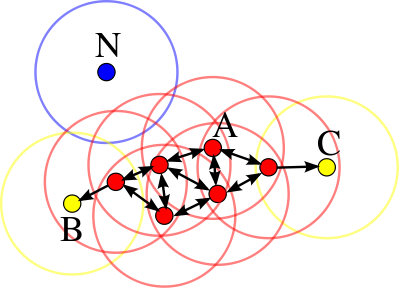
\includegraphics[width=.4\textwidth]{graphs/dbscan.png}
    \caption{The labels according to DBSCAN algorithm with minimum points is four, where the red dots are core points, yellow dots border points and blue dots anomalies. Core points are points that have within a certain distance a minimum amount of points. Border points don't have the minimum amount, but are within reach of a core point. Anomalies don't have the minimum amount of points in a certain area and are not reachable from a core point. (source: \url{https://en.wikipedia.org/wiki/DBSCAN})}
    \label{fig:dbscan}
\end{figure}

\subsubsection{Input variables}
%eps and minpts
According to \cite{ester1996density} we can set the minimum amount of points a core point needs in his area to four for two dimensional data. However for the area we need to calculate the radius, also called the eps variable. This eps is calculated by first calculating the distance to the fourth nearest neighbour for every point. These distances are then sorted and plotted. The value for eps can then be read from the graph looking at the first valley \cite{ester1996density}. In our implementation we calculated this eps automatically for every single program. To retrieve the first valley we looked at the differences between the slopes around a point. The point with the biggest difference in slopes was in the valley and was used as our eps variable for that specific program.\\

These two parameters have a big influences on how the clusters are divided and which points are labelled as an anomaly. When the minimum amount of points gets smaller more clusters will be formed and when it gets larger less clusters will be formed, assuming eps stays the same. When eps gets smaller more points will be labelled as anomalies and when eps get larger less points will be labelled as anomalies, assuming the minimum points parameter stays the same.

\subsection{Clustering}
%kmeans
When trying to find clusters in our data we were searching for a specific amount of clusters. Because the amount of clusters was known before clustering the k-means clustering algorithm was used. This algorithm begins by randomly assigning means for the amount of clusters specified. Then all the points are passed and divided into a cluster based on which mean has the shortest euclidean distance. After this the mean of the clusters is calculated and these will be the new means. This will iterate till a local maximum is found or the maximum amount of iterations has passed. The maximum amount of iterations was left to the default of 300 form the \textit{sklearn} python packages.


%compiler
%miss framewrok benchmark game
%energy uitleggen
%miss units uitleggen
%basic statistics: null hypothese, alpha, p, rejecting h0 more valuable